\section{On-demand open-world evaluation for KBP}
\label{sec:application}
Applying the on-demand open-world evaluation framework needs us to define 3 operations:
\begin{enumerate}
  \item Given some system output $X_i$, how should we sample its elements, i.e.\ what is $p_i(x)$?
  \item How do we verify system output, i.e.\ check if $x \in \sY$?
  \item How do we sample from the unknown set of true instances $x \sim \sY$?
\end{enumerate}
In this section, we'll see how each of these operations can be practically implemented for knowledge base population.

\subsection{Sampling from system predictions}
% 1. what is the point of this distribution?
% - prevent over sampling instances.
Recall that a KBP system predicts relational tuples of the form (\entity{subject}, \relation{predicate}, \entity{object}, \textsc{provenance}).
The choice of distribution over system predictions, $p_i(x)$, allows us to calibrate our precision metric to increase the representation of rare predicates or subject entities in our precision score.
This can desirable because, in practice, it is common for a system's predictions to be be dominated by a few common predicates (e.g.\ professional titles) or subject entities (like ``the United States of America''), skewing our evaluation metrics towards a particular relation or entity type.

The traditional solution to this problem is to take the macro average of the metric over predicates or subject entities.
We can replicate this behavior with the appropriate choice of a sampling distribution.
To estimate the macro-average over predicates, we use a predicate-centric distribution $p_i^\text{(p)}$ that first uniformly samples a predicate and then uniformly samples an instances with that predicate.
Similarly, to estimate the macro-average over subject entities, we use an entity-centric distribution $p_i^\text{(e)}$ that first uniformly samples over the entities in the system's predicted relational tuples and then uniformly samples instances with that entity as its subject.
Detailed histograms comparing different sampling distributions can be found in \appendixref{implementation}.

\begin{figure*}[t]
\begin{subfigure}{0.49\textwidth}
  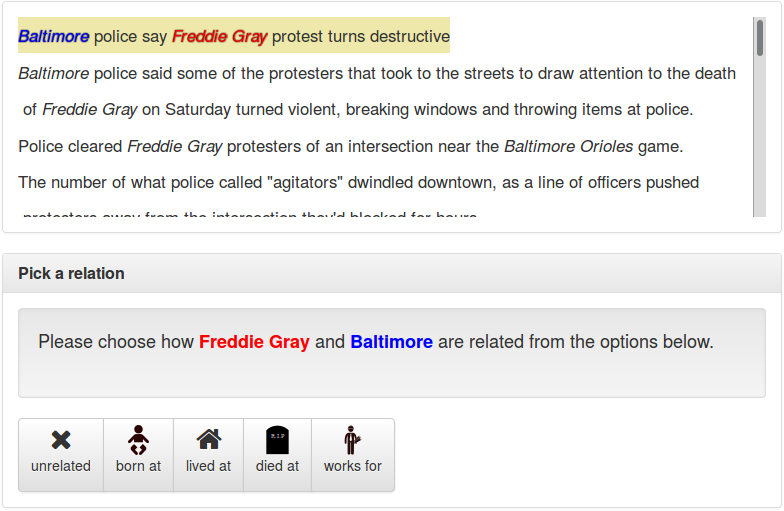
\includegraphics[width=\textwidth]{figures/interface/relation-interface}
  \caption{\label{fig:relation-interface} Relation extraction.}
\end{subfigure}
\hfill
\begin{subfigure}{0.49\textwidth}
  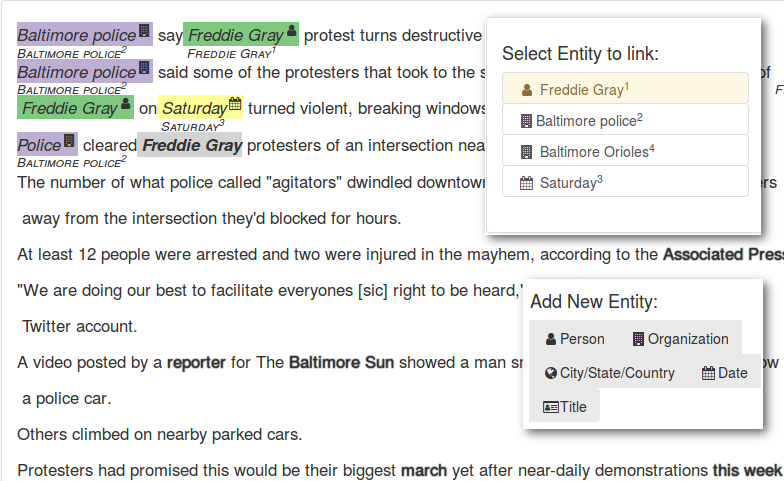
\includegraphics[width=\textwidth]{figures/interface/extraction-interface}
  \caption{\label{fig:entity-interface} Entity detection and linking.}
\end{subfigure}
\caption{\label{fig:interfaces} Screenshots of the annotation interfaces.}
\end{figure*}

\subsection{Verifying system predictions}
When verifying relational tuples predicted by a system, 
  crowd workers are presented the tuple's provenance and are asked to identify if a relation holds between the identified subject and object mentions (\reffig{relation-interface}). 
  Crowd workers also link the subject and object mentions to pages on Wikipedia, if possible.
On average, we find that crowdworkers are able to perform this task in about 30 seconds, corresponding to about \$0.10 per instance.
We requested 5 crowdworkers to annotate a small set of 200 relation instances from the 2015 TAC-KBP corpus 
and measured an inter-annotator agreement of 0.90 with 3 crowdworkers and 0.95 with 5.
Consequently, we take a majority vote over 3 workers in subsequent experiments, leading to a total cost of \$0.30 per relation.

\subsection{Sampling true instances}
Sampling from the set of true instances $\sY$ is difficult because we can not even enumerate the elements of $\sY$.
As a proxy, we assume that relations are identically distributed across documents and have crowd workers annotate a random subset of documents for relations.

To do so, crowd workers begin by identifying every mention span in a document and specifying its type.
  For each mention, they are also asked to identify the canonical mention within the document
  and identify links to Wikipedia pages where possible (\reffig{entity-interface}).
Finally, using a separate interface, crowdworkers annotate relations between pair of mentions within a sentence.

We compare crowdsourced annotations against those of expert annotators using data from the TAC-KBP 2015 EDL task on 100 documents~\citep{}.
Each document was annotated by at least 7 crowdworkers.
We find that 3 crowdworkers are together identify 92\% of the entity spans identified by expert annotators,
  and 7 crowdworkers together identify 96\%.
When using a token-level majority vote to identify entities, crowdworkers identify about 78\% of the entity spans; this number does not change significantly with additional crowdworkers.
We also measure substantial token-level inter annotator agreement for identifying typed mention spans ($\kappa = 0.83$), canonical mentions ($\kappa = 0.75$) and entity links ($\kappa = 0.75$) with just three workers.
Based on this analysis, we use token-level majority over 3 workers in subsequent experiments.

These interfaces are far more involved: the entity annotation interface takes on average about 13 minutes per document, corresponding to about \$2.60 per document, while the relation annotation interface takes on average about \$2.25 per document.
Because documents vary significantly in length and complexity, we set rewards for each document based on the number of tokens (.75c per token) and mention pairs (5c per pair) respectively.
With 3 workers per document, we paid on average about \$15 per document.
On average, each document contained 16.8 relations and it cost about \$0.87 per relation about three times as much as verifying a relation.

A final issue to discuss is how documents themselves should be sampled to capture diverse entities that span documents.
When considering uniformly sampled documents, we found that a majority of the relations extracted correspond to very rare entities and result in very few entities with more than one relation (\reffig{entity-distribution}).
In contrast, the TAC-KBP query are almost evenly split between rare and semi-frequent entities.
As a heuristic, we adopt the following two-stage sampling procedure:
First, 20\% of our exhaustive document collection is sampled uniformly and annotated.
We then uniformly sample the entities annotated to create a collection of ``query entities''.
Finally, we construct the remaining 80\% of our document collection by searching for documents that contain the query entities according to an exact string match. This process results in far more entities of medium frequency.
